\section{Discussion}

The results highlight how the vanilla REINFORCE algorithm struggled to 
discover a policy that allows the locomotion of the Hopper, achieving a 
low average reward during training (around $1006$) and displaying low test 
returns (ranging from $710$ to $1305$). As expected, this is due to the high 
variance of full-trajectory Monte Carlo returns, which causes noisy gradient 
updates leading to inefficient learning and slow convergence. Regarding 
training time, $57.6$ minutes was the fastest among the three, primarily 
driven by the short episode length ($178$ steps on average) caused by the 
agent frequently falling.

Introducing a constant baseline of $b{=}20$ had a positive impact on 
performance: the peak training average reached $1807$ and the best-performing 
seed achieved a mean test return of $2444$. The baseline reduces the variance 
of the gradient estimates by subtracting a fixed offset from the Monte Carlo 
return, which also improved the average episode length from $178$ to $215$ 
steps, reflected in the higher training time of $70.3$ minutes. 

In principle, 
a good baseline should approximate the expected return, given that vanilla 
REINFORCE achieved a mean training reward of around $1006$, the chosen value 
of $b{=}20$ is far from this optimum, meaning that the variance reduction 
achieved is real but limited.


While a constant baseline ($b=20$) reduced variance and improved performance over vanilla REINFORCE, it applies a global correction that is identical across all states. Actor-Critic further improved stability by using a state-dependent baseline $V(s)$, which adapts to the local structure of the value function, providing a much more effective variance reduction at each step.



The results obtained in the first part demonstrate that the proposed Actor-Critic framework successfully learned a locomotion policy for the Hopper environment.
Nevertheless, training did not fully converge to stable hopping: significant reward variance remained throughout the final stages of training, 
indicating still high exploration and stochasticity, preventing the Hopper to reproduce its best behaviors consistently.

This result represents a substantial improvement compared to embryonic versions of Actor-Critic implementations, as they 
converged to a "lazy" standing-still policy. This can mathematically occur due to an agent maximizing only the survival component of the reward function.

% Standing actions were continuously selected as they tended to achieve high positive advantages, while jumping actions
% consistently turned out to be worse than the critic’s expectations.
% This occurred due to the initial usage of the TD(0) target, in which only the immediate subsequent
% state was considered, so jumping actions always led to immediate worse states, making them less appealing to a
% short-sighted critic and discouraging their exploration.
% Therefore, the short-sighted critic reinforced actions that led to immediate better states: standing,
% which continued to return a positive reward thanks to the survival component of the reward function, forcing the
% Hopper to adopt a reward-exploiting local optimum behavior.

Standing actions were continuously selected as they tended to achieve high positive advantages, while jumping actions
consistently turned out to be worse than the critic’s expectations. Because the initial TD(0) target only considered
the immediate next state, jumping appeared less rewarding and was therefore discouraged. As a result, the critic
reinforced standing behaviors, causing the Hopper to converge to a reward-exploiting local optimum based on the
survival component of the reward function.


The introduction of GAE, a sigma floor together with all the previously cited modifications, improved exploration and enabled
the policy to eventually discover hopping.

The final model's behavioral instability seems to be supported by the critic-loss spikes, which, however, 
should not necessarily be interpreted as training failure.
% These spikes are not necessarily indicative of unstable training as reinforcement-learning targets
% continuously change together with the current policy, therefore when the actor discovers substantially better trajectories,
% previously learned value estimates become obsolete and inaccurate, generating large temporal-difference errors and
% consequently large critic-loss spikes.
These spikes are not necessarily indicative of unstable training, since reinforcement-learning targets evolve together
with the policy. Therefore, when the actor discovers better trajectories, previously learned value estimates become inaccurate,
generating large temporal-difference errors and consequently critic-loss spikes.

In contrast, actor updates remained remarkably stable throughout training, as advantage normalization successfully bounded
policy updates and prevented gradient explosions.

Despite these improvements, the final policy still exhibits variability and has not fully converged. Future work
could investigate additional stabilization techniques like TRPO or PPO \cite{SchulmanTRPO2015, SchulmanPPO2017} and
more advanced actor-critic methods for continuous control, such as DDPG and TD3 \cite{Fujimoto2018}.

\subsection{Domain randomization on PandaPush}
SAC solves the push task almost converging on the source ($98.5\%$), and even the naive
source$\to$target transfer keeps a $97.5\%$ success rate, only marginally below the
target$\to$target upper bound: the injected mass shift ($1\!\to\!5$ kg) is a \emph{small}
reality gap for an off-policy learner with a replay buffer.
Success rate is already saturated, so UDR and ADR mainly improve the mean return (UDR $-0.509$ vs.\ the $-0.633$ lower
bound, closing $\sim\!66\%$ of the gap toward the $-0.445$ upper bound).
The mass-sensitivity sweep (Fig.~\ref{fig:sensitivity}) confirms this:
the non-randomized policy already generalises across a wide range of cube masses, leaving limited headroom for randomization.
This is the main limitation of the simplified sim-to-sim setting: when the source learner is strong,
domain randomization adds a robustness margin rather than rescuing a failing policy.
UDR can also fall into a conservativism trap when its range is too wide.
On the other hand ADR removes the manual range at the cost of extra sampling-schedule hyperparameters (boundary thresholds and step size).


\begin{figure}[htbp]
    \centering
    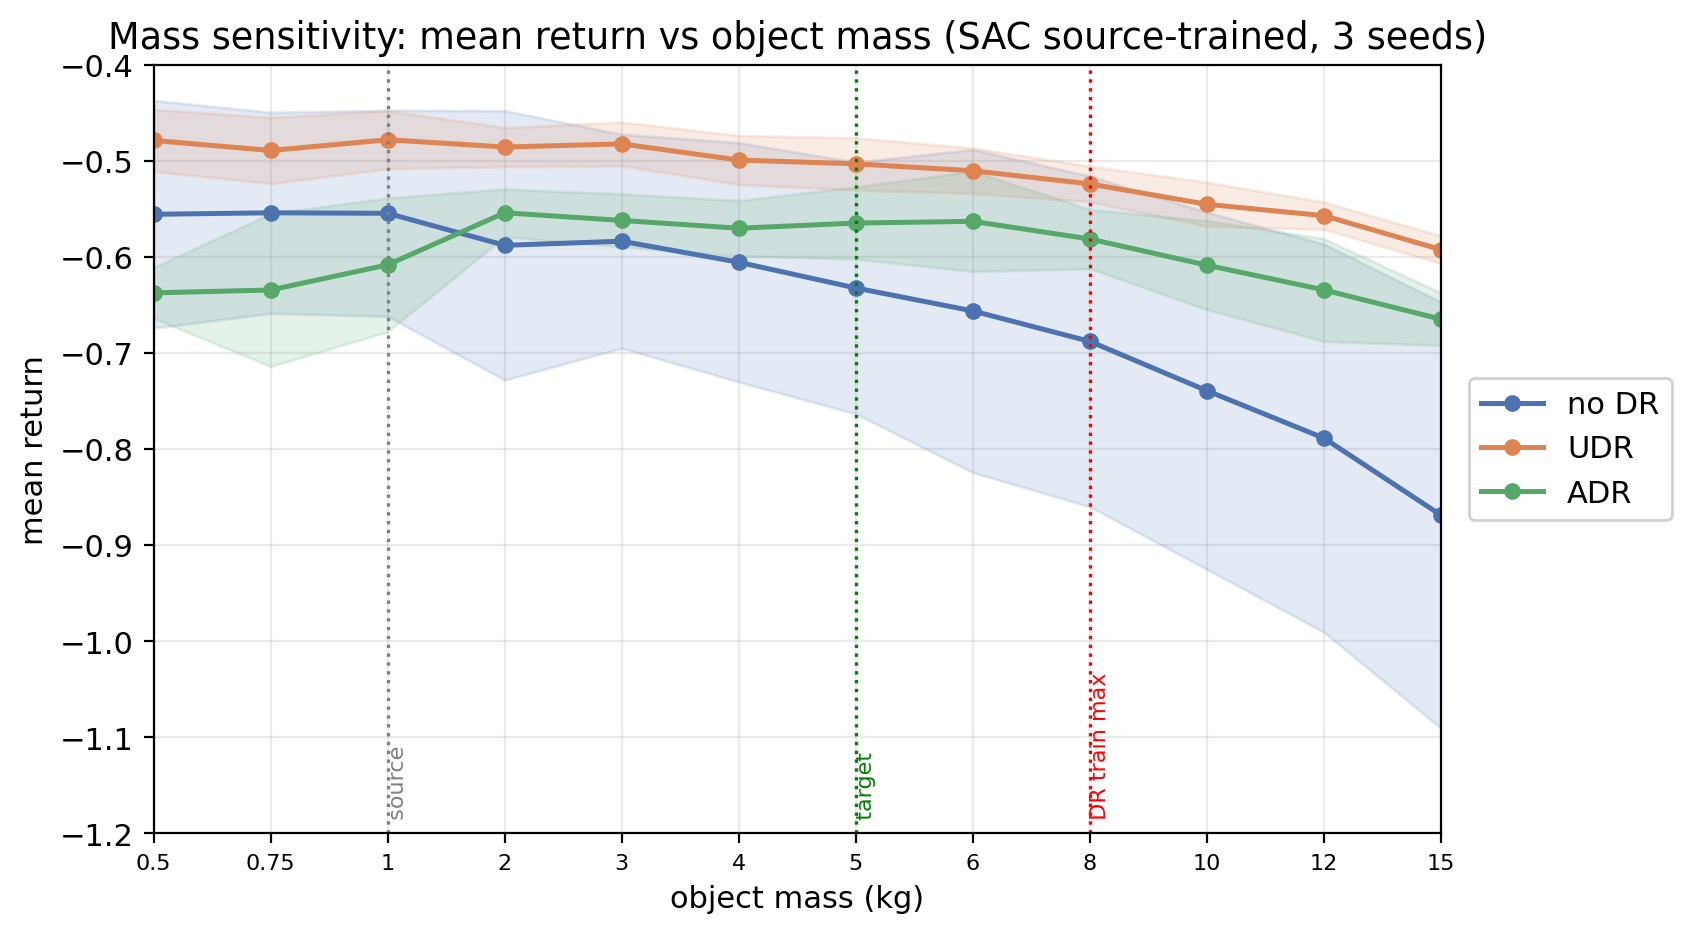
\includegraphics[width=\columnwidth]{imgs/sensitivity_return.png}
    \caption{Mass-sensitivity analysis.}
    \label{fig:sensitivity}
\end{figure}